\documentclass[12pt]{article}

\usepackage{amssymb,amsmath,amsfonts, booktabs, dsfont, eurosym,float,geometry,ulem,graphicx,caption,color,setspace,sectsty,comment,footmisc,caption,multicol, multirow, natbib, pdflscape,array,hyperref}
\bibliographystyle{rusnat}


\normalem

\geometry{left=0.5in,right=0.5in,top=1.0in,bottom=1.0in}

\begin{document}



\begin{titlepage}
\title{Arjun Shanmugam's Senior Thesis}
\author{Arjun Shanmugam}
\date{\today}
\maketitle
\begin{abstract}
\noindent Placeholder\\

\bigskip
\end{abstract}
\setcounter{page}{0}
\thispagestyle{empty}
\end{titlepage}
\pagebreak \newpage

\doublespacing

\section{Introduction} \label{sec:introduction}
\bibliography{writing/paper/citations}
\subsection{Literature Review}

\section{Institutional Context}
    \subsection{Eviction in Massachusetts}
        \subsubsection{The Massachusetts Housing Court}
        \subsubsection{The Eviction Process}
    \subsection{Property Tax Assessment}
        \subsubsection{The Property Value Assessment Process}
    \subsection{Zestimates}
        \subsubsection{How Are Zestimates Produced?}
        \subsubsection{Reliability}
\section{Data} \label{sec:data}
    \begin{landscape}
    \subsection{Evictions Data}
        \begin{figure}[H]
            \centering
            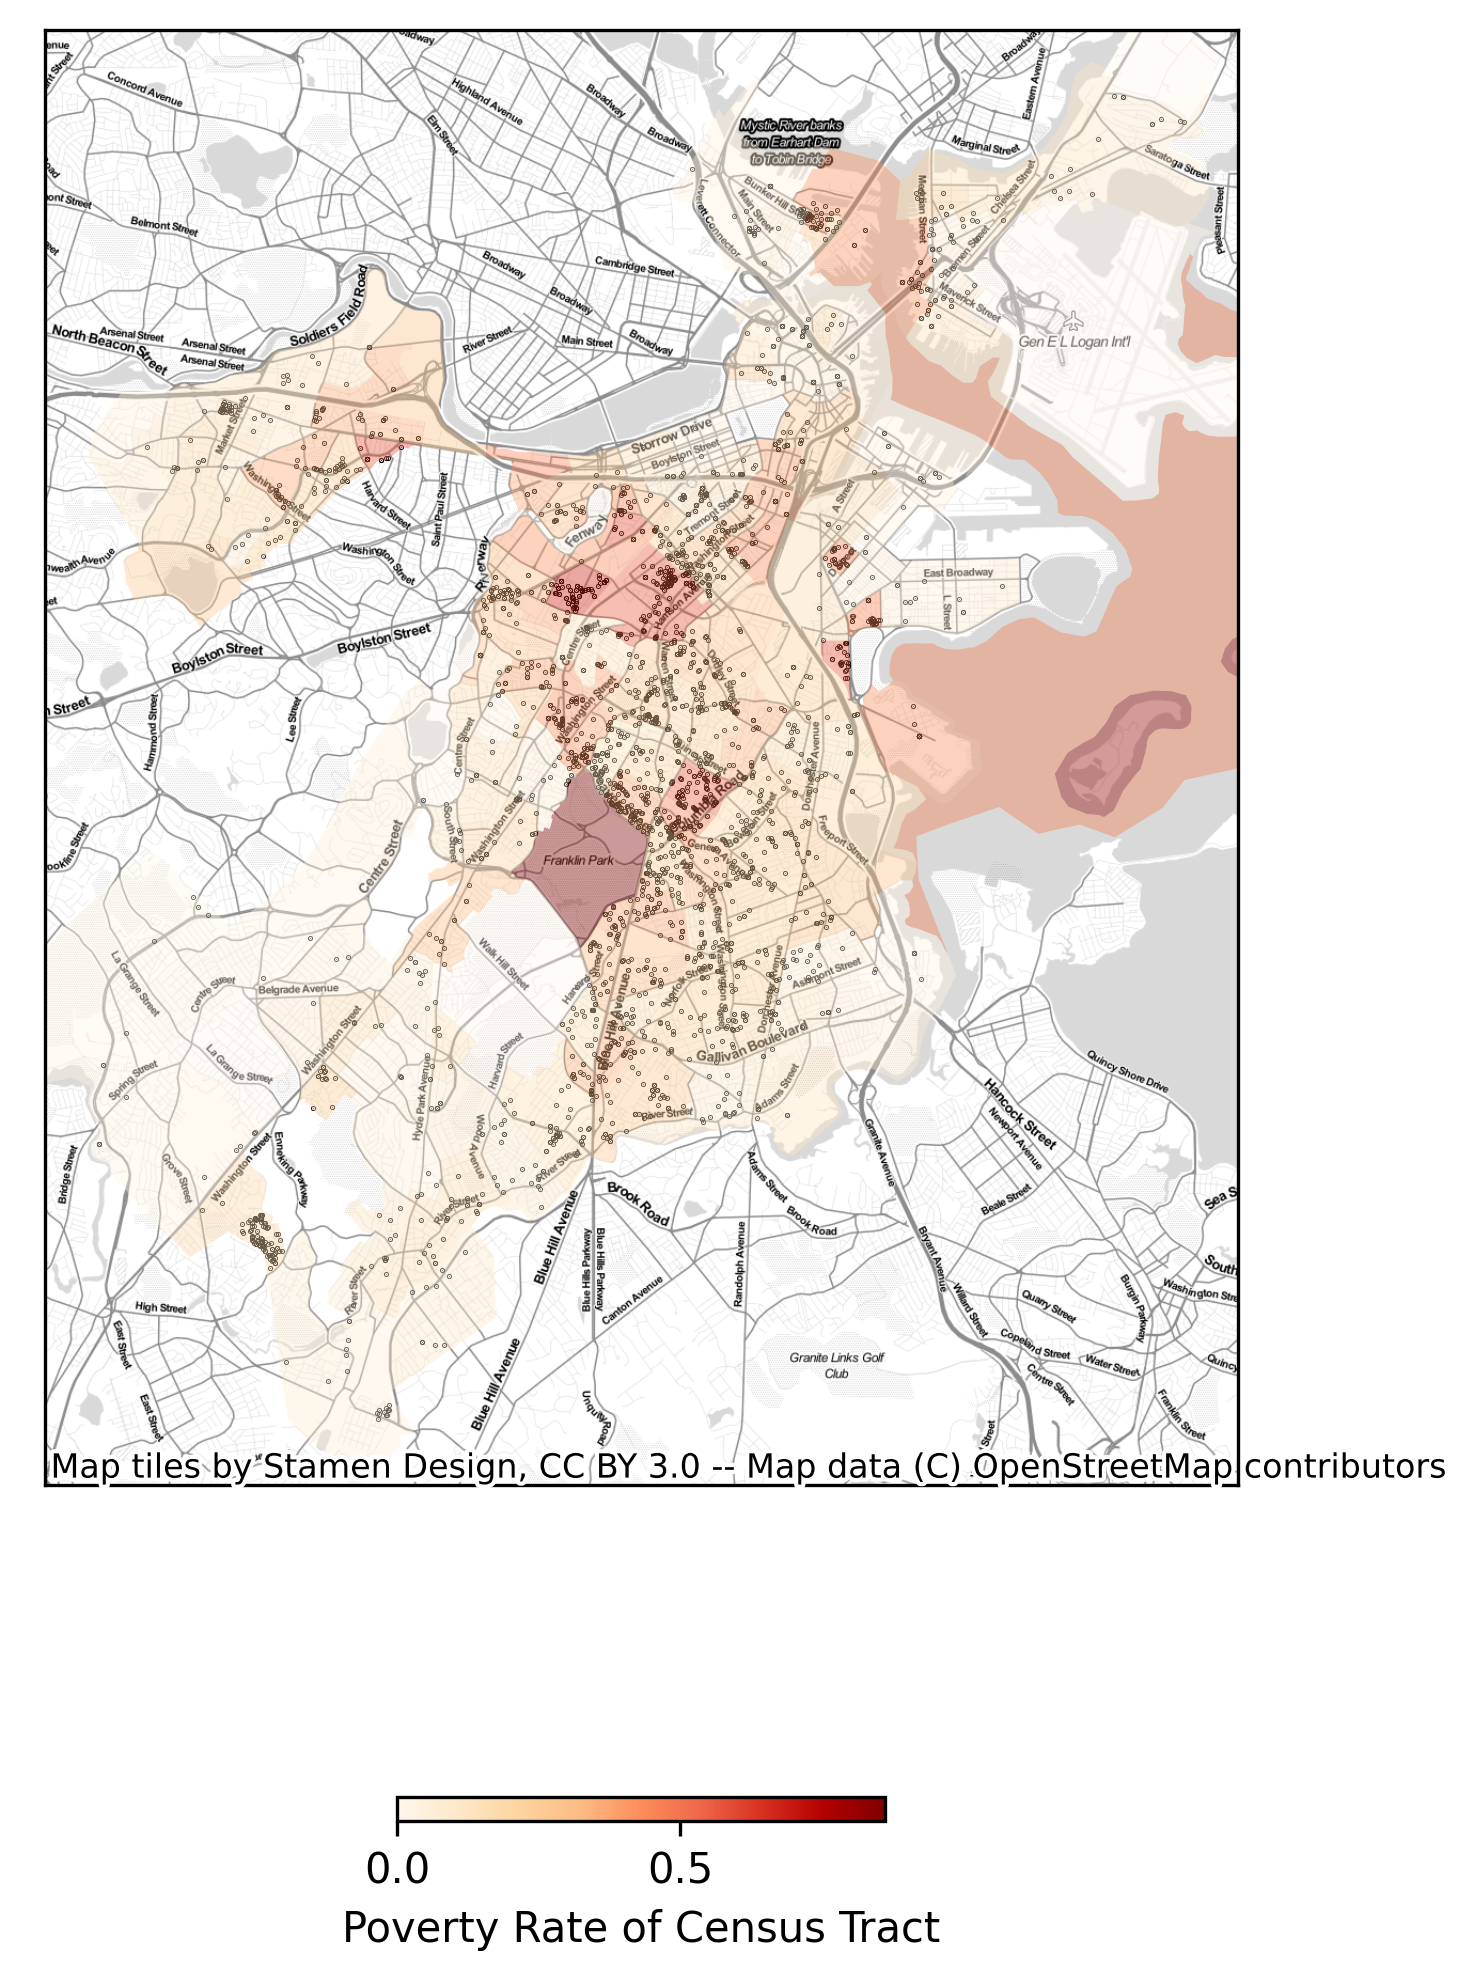
\includegraphics{output/summary_statistics/figures/evictions_map.png}
            \caption{Spatial Incidence of Eviction}
            \label{fig:my_label}
        \end{figure}

        \begin{figure}[H]
            \centering
            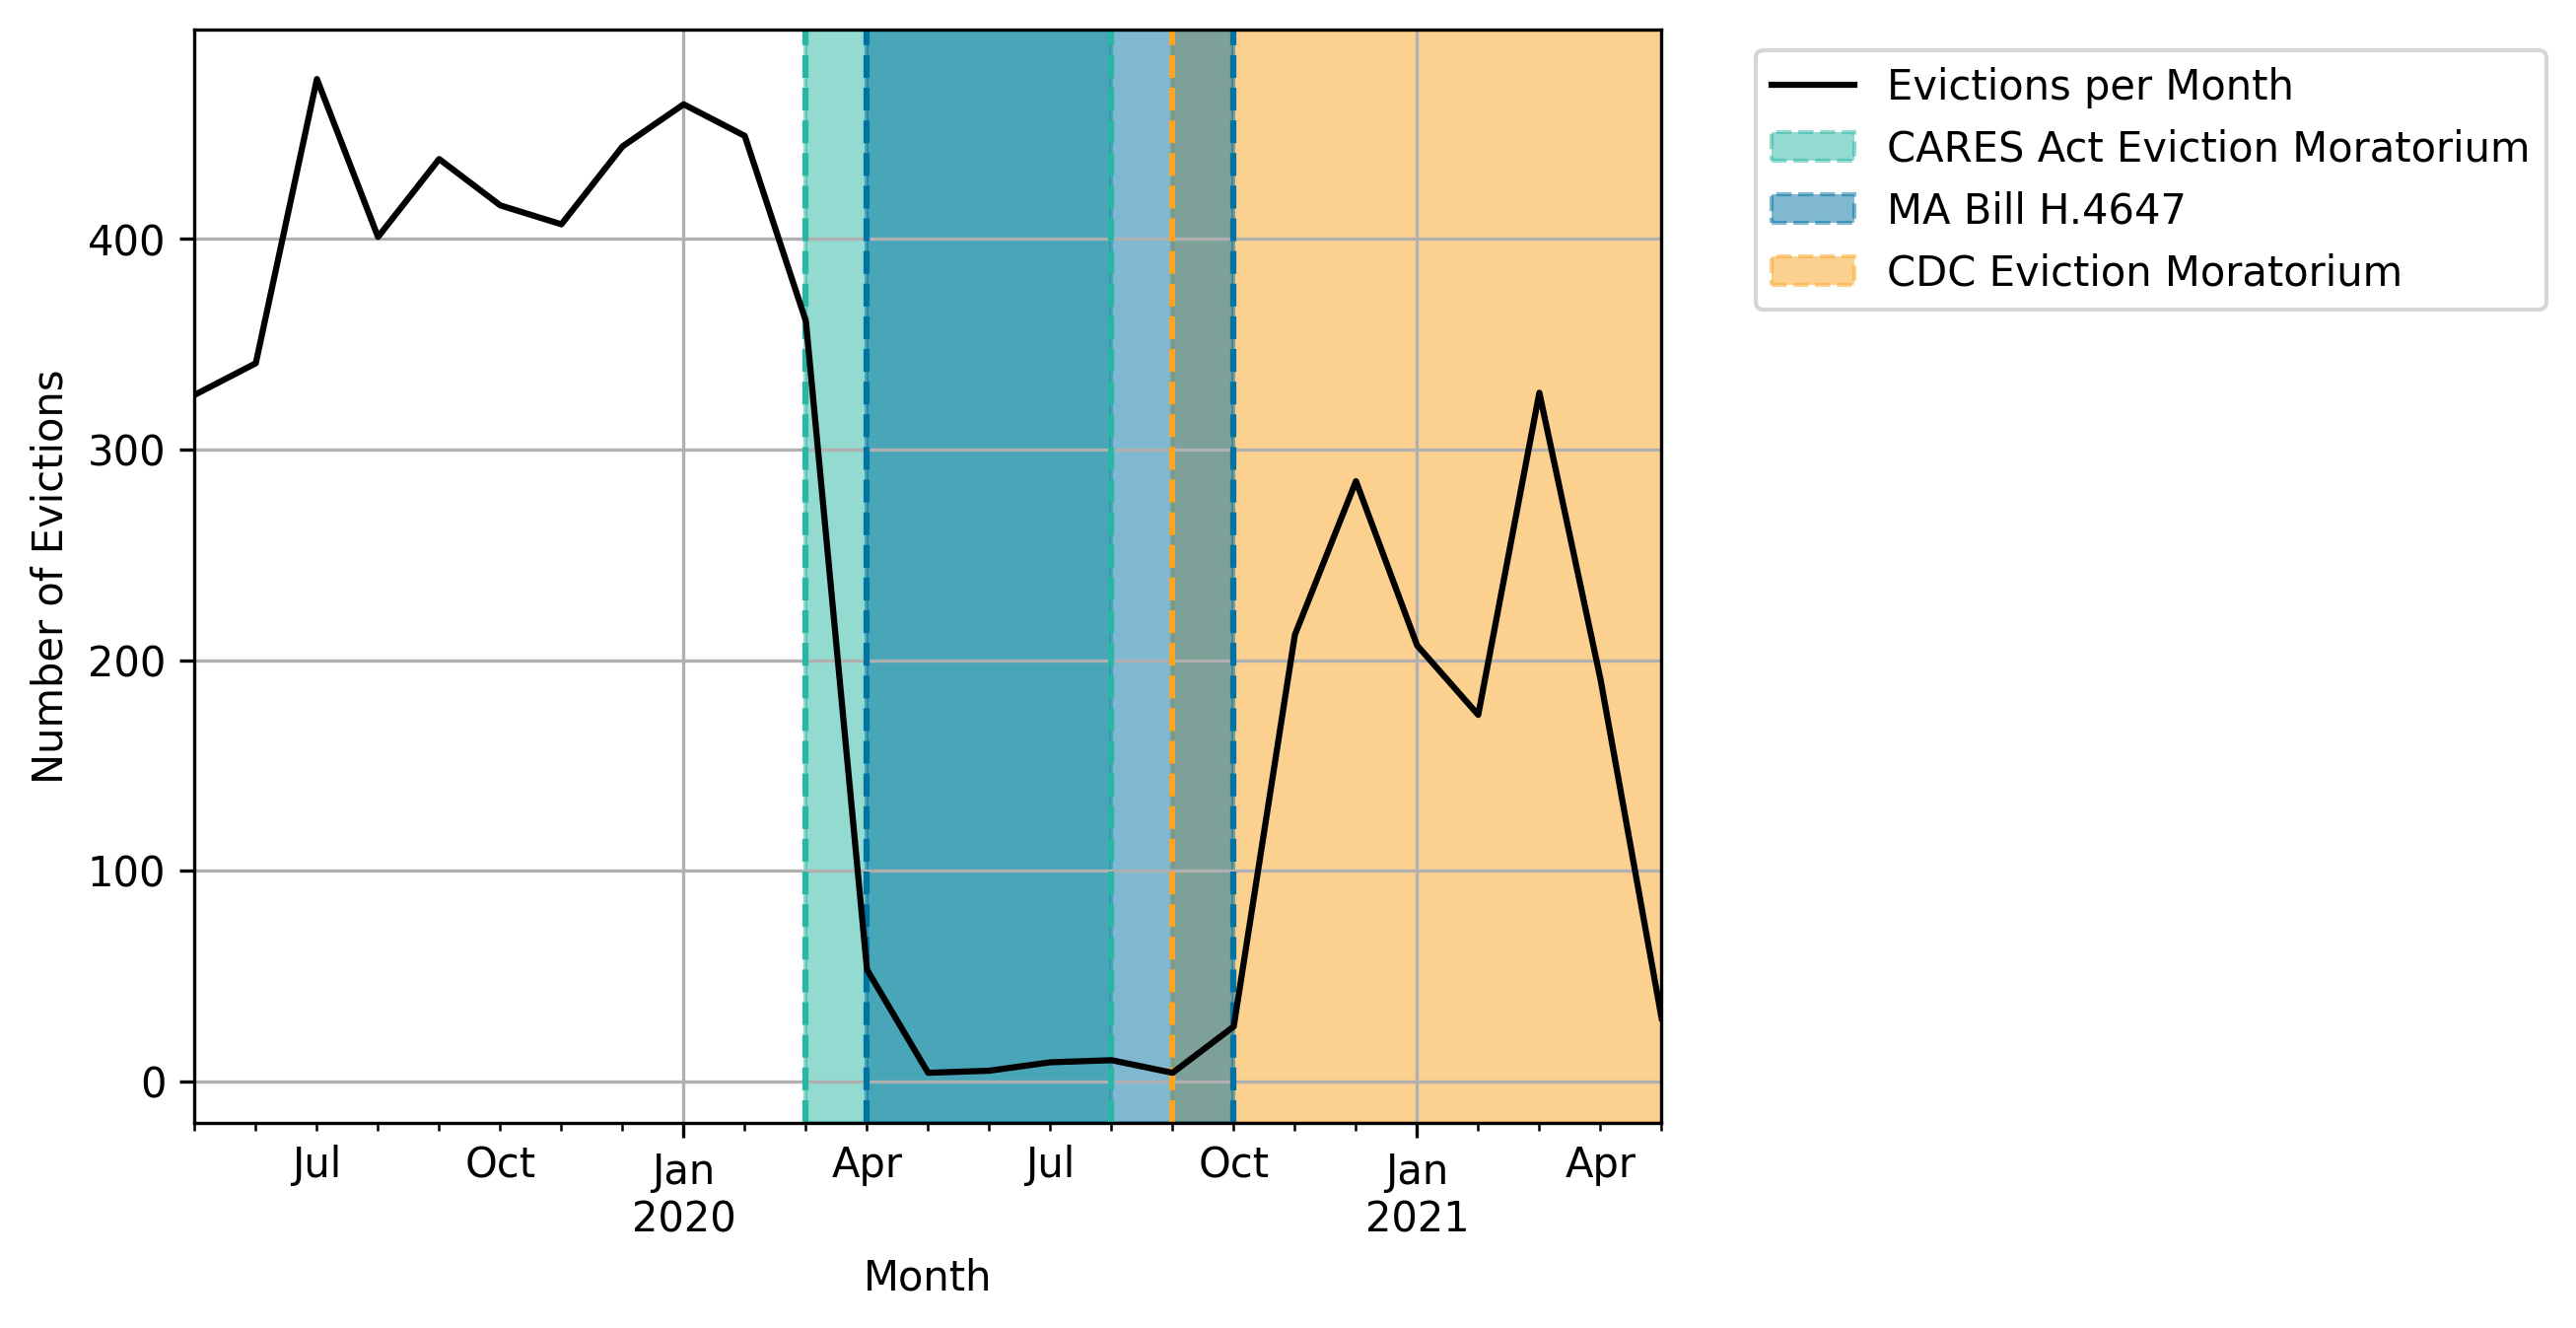
\includegraphics{output/summary_statistics/figures/filings_over_time.png}
            \caption{Eviction Filings Over Time}
            \label{fig:my_label}
        \end{figure}
    \end{landscape}
        \begin{table}[H]
            \centering
            \begin{tabular}{lccc}
\toprule
 & Cases Won By Defendant & Cases Won By Plaintiff & Portion of All Cases \\
\midrule
All Filing Dates & 858 & 2,440 & 1.00 \\
2019-05 & 100 & 156 & 0.08 \\
2019-06 & 38 & 151 & 0.06 \\
2019-07 & 42 & 198 & 0.07 \\
2019-08 & 31 & 178 & 0.06 \\
2019-09 & 37 & 156 & 0.06 \\
2019-10 & 33 & 148 & 0.05 \\
2019-11 & 23 & 138 & 0.05 \\
2019-12 & 28 & 171 & 0.06 \\
2020-01 & 17 & 159 & 0.05 \\
2020-02 & 38 & 139 & 0.05 \\
2020-03 & 70 & 85 & 0.05 \\
2020-04 & 14 & 19 & 0.01 \\
2020-05 & 0 & 1 & 0.00 \\
2020-06 & 2 & 2 & 0.00 \\
2020-07 & 1 & 2 & 0.00 \\
2020-08 & 1 & 2 & 0.00 \\
2020-09 & 1 & 6 & 0.00 \\
2020-10 & 7 & 14 & 0.01 \\
2020-11 & 54 & 151 & 0.06 \\
2020-12 & 71 & 159 & 0.07 \\
2021-01 & 81 & 120 & 0.06 \\
2021-02 & 58 & 86 & 0.04 \\
2021-03 & 58 & 89 & 0.04 \\
2021-04 & 45 & 93 & 0.04 \\
2021-05 & 8 & 17 & 0.01 \\
\bottomrule
\end{tabular}

            \caption{Distribution of Eviction Filings and Outcomes}
            \label{tab:my_label}
        \end{table}

        \begin{figure}[H]
            \centering
            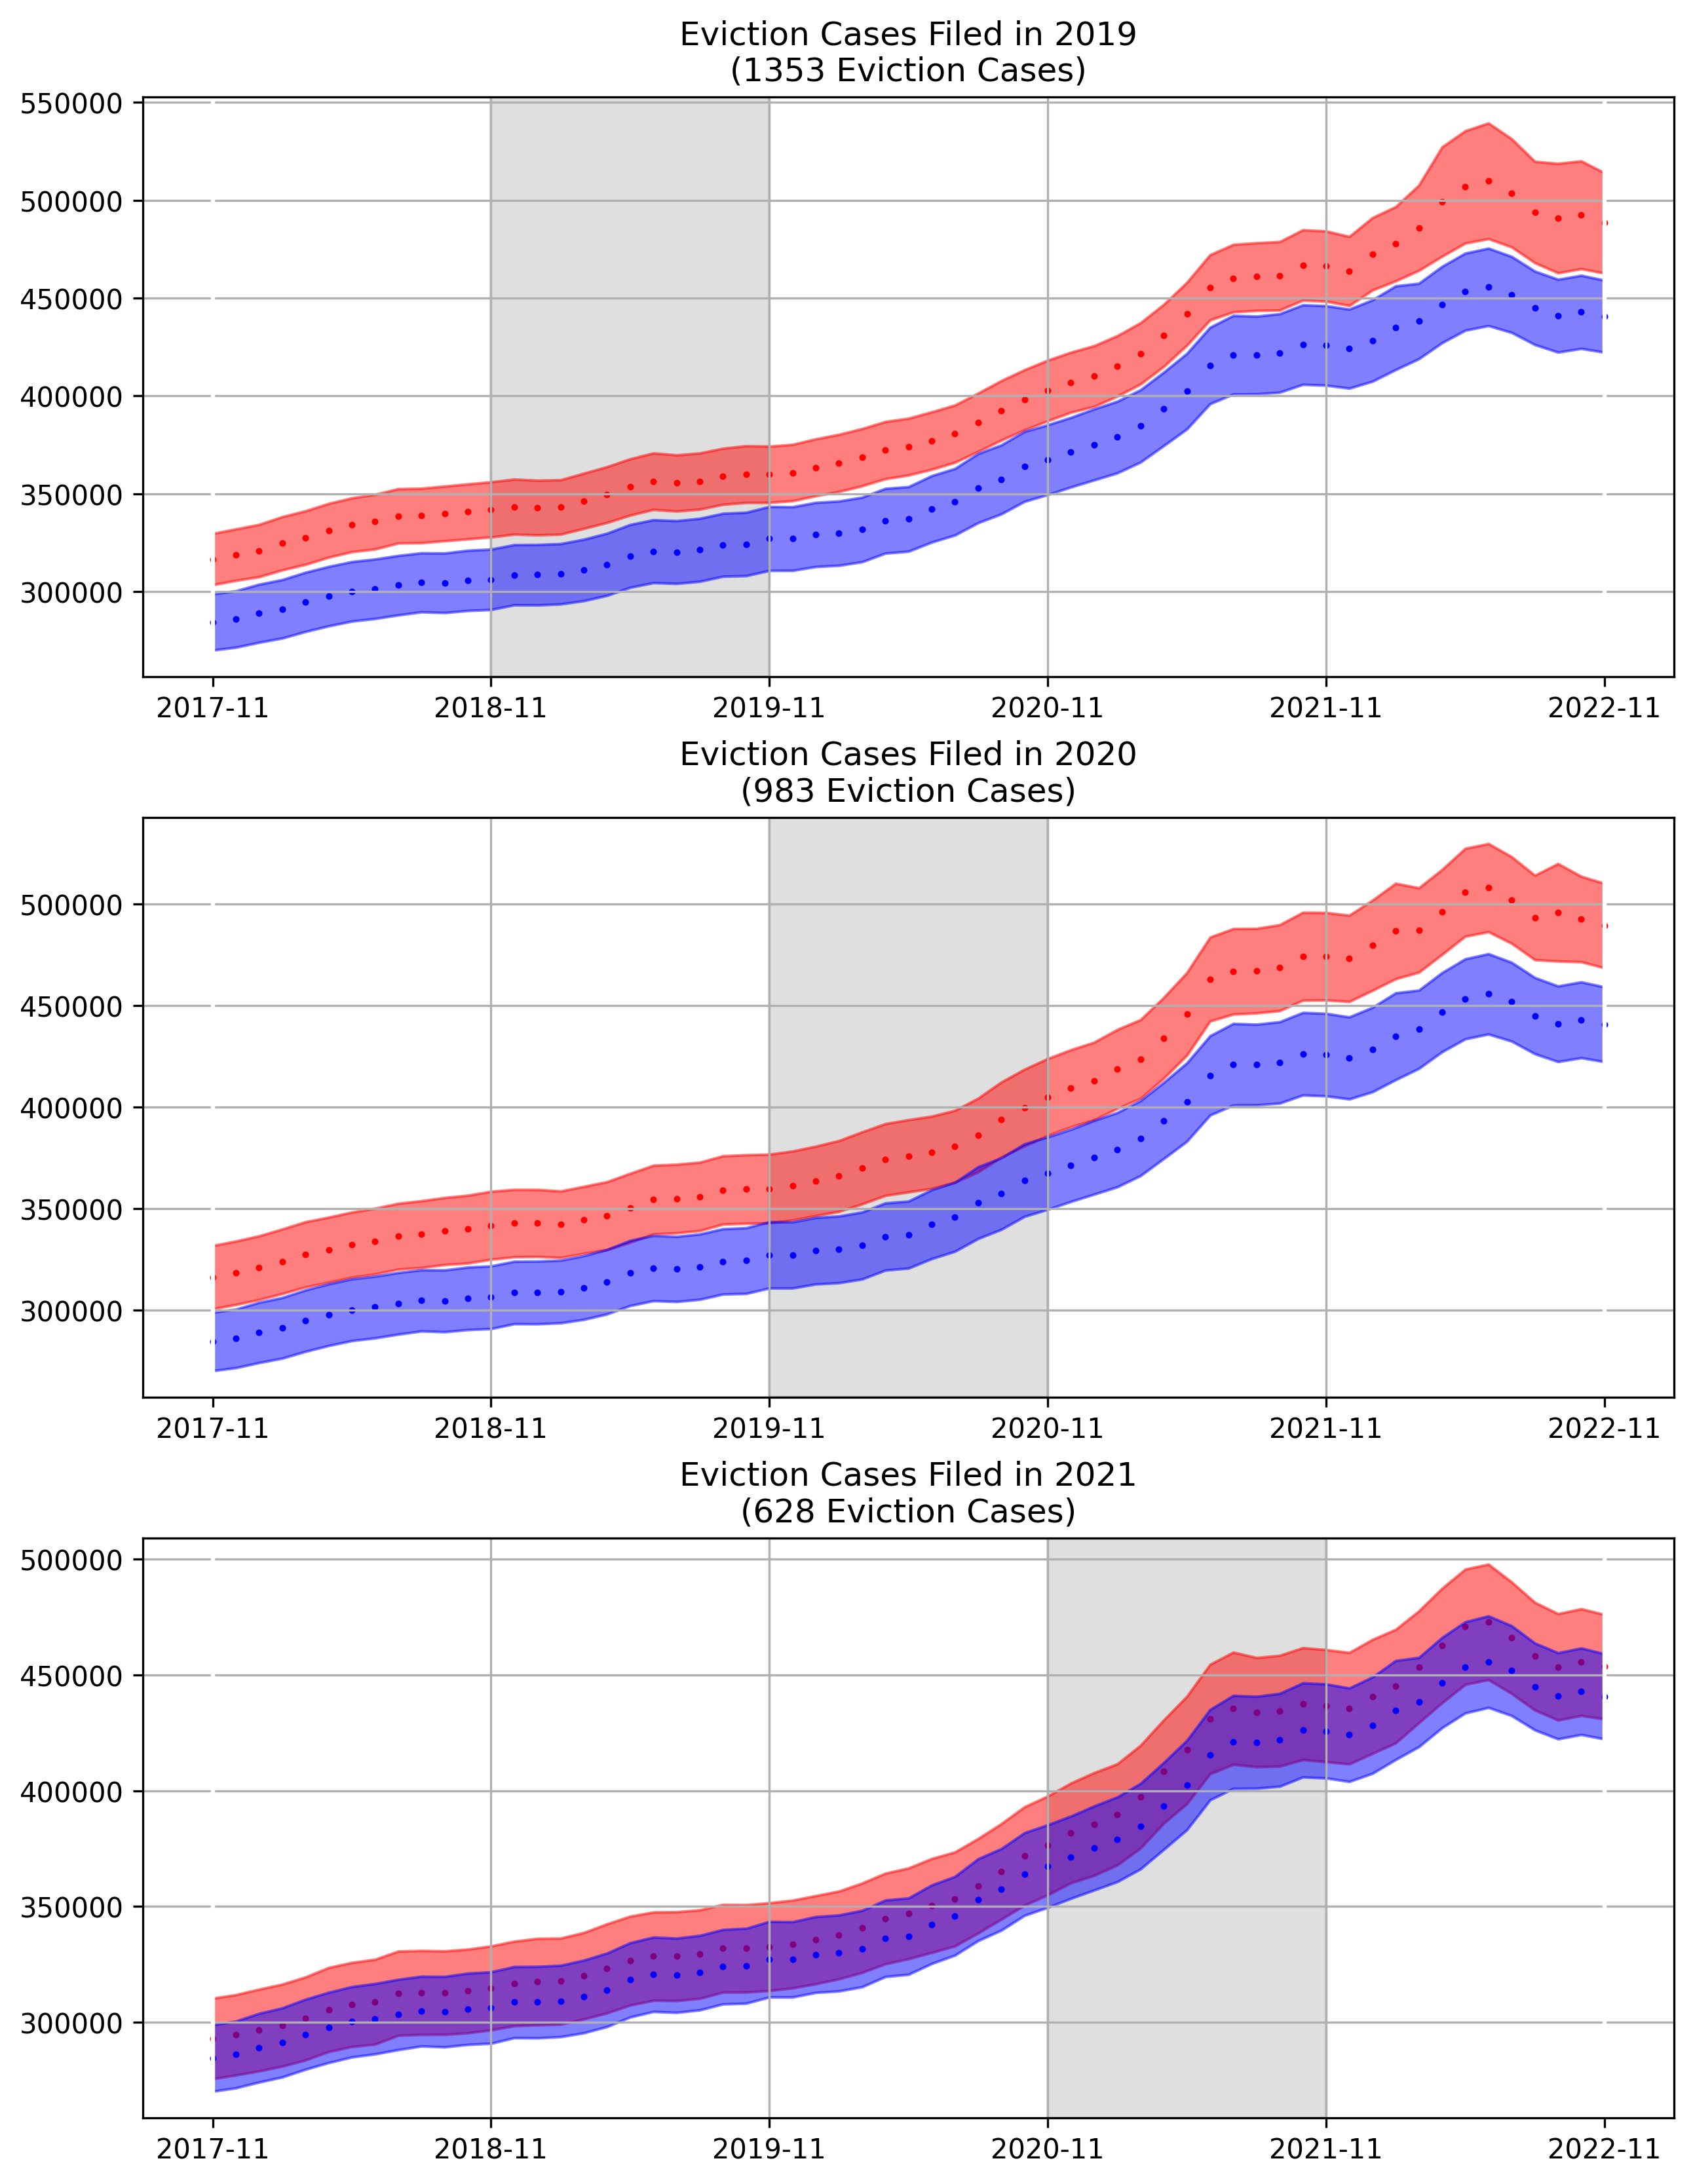
\includegraphics[scale=0.8]{output/DiD/figures/trends_in_zestimates_by_cohort.png}
            \caption{Trends in Zestimates by Cohort}
            \label{fig:my_label}
        \end{figure}

    \subsection{Summary Statistics}
         \begin{table}[H]
            \centering
            \small
            \begin{tabular}{llcccc}
\toprule
 &  & Mean & Median & S.D. & N \\
Panel & Variable &  &  &  &  \\
\midrule
\multirow[c]{3}{4cm}{\textit{Panel A: Case Initiation}} & For cause & 0.12 & 0.00 & 0.33 & 40,727 \\
 & No cause & 0.11 & 0.00 & 0.31 & 40,727 \\
 & Non-payment of rent & 0.75 & 1.00 & 0.43 & 40,727 \\
\cline{1-6}
\multirow[c]{6}{4cm}{\textit{Panel B: Case Resolution}} & Case defaulted & 0.20 & 0.00 & 0.40 & 40,727 \\
 & Case dismised & 0.29 & 0.00 & 0.45 & 40,727 \\
 & Case duration & 57.81 & 21.00 & 78.29 & 39,087 \\
 & Case heard & 0.06 & 0.00 & 0.23 & 40,727 \\
 & Case mediated & 0.41 & 0.00 & 0.49 & 40,727 \\
 & Money judgment & 1,890.34 & 0.00 & 5,279.49 & 40,727 \\
\cline{1-6}
\multirow[c]{4}{4cm}{\textit{Panel C: Defendant and Plaintiff Characteristics}} & Defendant has an attorney & 0.09 & 0.00 & 0.28 & 40,727 \\
 & Defendant is an entity & 0.01 & 0.00 & 0.08 & 40,727 \\
 & Plaintiff has an attorney & 0.84 & 1.00 & 0.37 & 40,727 \\
 & Plaintiff is an entity & 0.70 & 1.00 & 0.46 & 40,727 \\
\cline{1-6}
\multirow[c]{4}{4cm}{\textit{Panel D: Assessor Records From Most Recent Pre-Filing F.Y.}} & Building value & 8,350,204.19 & 636,500.00 & 22,073,916.94 & 36,587 \\
 & Land value & 2,471,065.61 & 192,400.00 & 6,218,383.08 & 36,587 \\
 & Other value & 112,575.80 & 1,000.00 & 659,661.29 & 36,587 \\
 & Total property value & 10,900,678.30 & 954,900.00 & 26,482,630.60 & 36,587 \\
\cline{1-6}
\multirow[c]{4}{4cm}{\textit{Panel E: Census Tract Characteristics}} & Median household income (2016) & 52,659.44 & 47,105.00 & 27,177.48 & 40,726 \\
 & Median two bedroom rent (2015) & 1,116.27 & 1,055.00 & 396.29 & 30,537 \\
 & Population density (2010) & 9,159.77 & 5,978.61 & 9,574.14 & 40,726 \\
 & Portion white (2010) & 0.58 & 0.63 & 0.29 & 40,726 \\
\cline{1-6}
\multirow[c]{9}{4cm}{\textit{Panel F: Zestimates Around Filing Date}} & Filing date & 377,384.02 & 305,144.00 & 316,645.29 & 10,096 \\
 & Five years before filing date & 261,462.86 & 213,270.60 & 238,040.64 & 9,842 \\
 & Four years before filing date & 280,243.32 & 225,065.75 & 276,051.45 & 9,968 \\
 & One year after filing date & 421,601.75 & 347,550.00 & 344,328.86 & 10,443 \\
 & One year before filing date & 351,172.05 & 278,722.25 & 311,982.74 & 10,190 \\
 & Three years after filing date & 501,611.80 & 414,600.00 & 780,467.01 & 5,894 \\
 & Three years before filing date & 307,137.16 & 240,097.38 & 369,763.53 & 10,172 \\
 & Two years after filing date & 477,948.08 & 393,900.00 & 457,694.83 & 9,175 \\
 & Two years before filing date & 341,084.08 & 259,176.00 & 987,145.51 & 10,182 \\
\cline{1-6}
\bottomrule
\end{tabular}

            \caption{Summary Statistics}
            \label{tab:table_1}
        \end{table}
        \newpage

\section{Empirical Strategy: Difference-in-Differences}
    I seek to estimate the average treatment effects of plaintiff victory in eviction cases on treated properties. I use the staggered difference-in-difference estimator proposed in \cite{callaway_difference--differences_2021}, which uses two-period, two-unit difference-in-difference estimators to estimate time- and cohort-specific ATTs and then aggregates them, weighting by cohort size, to produce summaries of the ATT. 
    
    
    Let $G_i$ be the month during which the eviction case involving property $i$ was filed, such that $G_i = g \in \{\text{May} \; 2019, \text{June} \; 2019, ..., \text{May} \; 2021\}$. Let $C_i = 1$ if the eviction case involving $i$ resulted in a victory for the defendant and $0$ otherwise. If $G_i = g$ and $C_i = 0$, then property $i$ is a treated property and a member of the cohort first treated during month $g$ (cohort $g$). If $C_i=1$, then property $i$ is a never-treated property. Let $Y_{i,t}$ be property $i$'s Zestimate during month $t$ and define $\Delta Y_{i, g-1, t} \equiv Y_{i,t} - Y_{i,g-1}$ so that $\Delta Y_{i, g-1, t}$ is the change in property $i$'s Zestimate between months $t$ and $g-1$.

    \subsection{Unconditional Estimates of the ATT}
    The following is an unconditional estimator for $ATT(g,t)$, the average treatment affect during month $t$ for cohort $g$.
    \begin{align}
        \hat{ATT}^{nev}_{un}(g, t) = \frac{\sum_i\Delta Y_{i, g-1, t}\mathds{1}\{G_i=g\}}{\sum_i\mathds{1}\{G_i=g\}} - \frac{\sum_i\Delta Y_{i, g-1, t}\mathds{1}\{C_i=1\}}{\sum_i\mathds{1}\{C_i=1\}}
    \end{align}
    The above estimator will identify $ATT(g,t)$ under the assumption that the change in untreated potential outcomes between periods $g-1$ and $t$ is the same among units in cohort $g$ as it is among never-treated units.

    \subsection{D.R. Estimates of the ATT}

    The above unconditional parallel trends assumption is unlikely to hold, as eviction case outcomes and zestimates may be related to their socioeconomic surroundings. Table 3 explores this theory further, reporting results from univariate regressions of January 2022 Zestimates and an indicator for plaintiff victory on the pre-treatment characteristics listed in Panels A through D of Table 2. Each cell gives the p-value from a regression of the variable which labels its column on the variable which labels its row. Table 3 shows significant associations between pre-treatment characteristics and Zestimates and pre-treatment characteristics and case outcomes, suggesting that the unconditional parallel trends assumption imposed earlier may not be valid.

    \begin{table}[H]
        \centering
        \begin{tabular}{llcc}
\toprule
 &  & \multicolumn{2}{c}{\textit{Dependent Variable}} \\
\cline{3-4}
\\
 &  & Zestimate, Dec. 2022 & Plaintiff victory \\
 & \emph{Independent Variable} &  &  \\
\midrule
\multirow[c]{2}{3cm}{\textit{Panel A: Pre-treatment Zestimates}} & Zestimate, Jan. 2017 & 0.00 & 0.00 \\
 & Change, Jan. 2017 to Jan. 2019 & 0.00 & 0.27 \\
\cline{1-4}
\multirow[c]{8}{3cm}{\textit{Panel B: Census Tract Characteristics}} & Share with bachelor's degree & 0.00 & 0.07 \\
 & Jobs per square mile (2010) & 0.00 & 0.63 \\
 & Median household income (2016) & 0.00 & 0.01 \\
 & Share below poverty line & 0.70 & 0.01 \\
 & Population density (2010) & 0.00 & 0.01 \\
 & Median two bedroom rent (2015) & 0.00 & 0.05 \\
 & Share white (2010) & 0.00 & 0.00 \\
 & Share with commute $<$15 minutes (2010) & 0.00 & 0.02 \\
\cline{1-4}
\multirow[c]{3}{3cm}{\textit{Panel C: Case Initiation}} & For cause & 0.01 & 0.68 \\
 & No cause & 0.98 & 0.03 \\
 & Non-payment of rent & 0.31 & 0.77 \\
\cline{1-4}
\multirow[c]{4}{3cm}{\textit{Panel D: Defendant and Plaintiff Characteristics}} & Defendant has an attorney & 0.37 & 0.00 \\
 & Plaintiff has an attorney & 0.61 & 0.47 \\
 & Defendant is an entity & 0.02 & 0.37 \\
 & Plaintiff is an entity & 0.62 & 0.13 \\
\cline{1-4}
\bottomrule
\end{tabular}

        \caption{Relationship Between Pre-Treatment Characteristics and the Dependent and Independent Variables}
        \label{tab:my_label}
    \end{table}

    My next strategy uses covariates to construct a more credible counterfactual for the observed path of outcomes in the treatment group using the doubly robust difference-in-differences estimator proposed by \cite{santanna_doubly_2018}. For each property, let $X_i$ be a vector containing the covariates whose univariate regression coefficients from column 1 of table 3 are significant at the 5 percent level. To attempt to identify $ATT(g, t)$ using the doubly robust estimator, I first estimate $\hat{p}_g(X_i)$, a logit regression propensity score model for being in cohort $g$. I assign a weight $\hat{w}_i(X_i) \equiv\frac{\hat{p}_g(X_i)}{1 - \hat{p}_g(X_i)}$ to each never-treated property $i$; $\hat{w}_i(X_i) \equiv 1$ for treated properties. Define $\hat{w}^*_i(X_i) = \frac{\hat{w}_i(X_i)}{\sum_i \hat{w}_i(X_i)}$. Second, using only never-treated counties, I regress $\Delta Y_{i, g-1, t}$ on $X_j$, weighting by $\hat{w}_i(X_i)$. Using the estimated coefficients $\hat{\beta}_{g-1, t}^{X}$, I define $\Delta \hat{\mu}_{g-1, t}(X_i) \equiv \hat{\beta}_{g-1, t}^{X}X_i$ so that $\Delta \hat{\mu}_{g-1, t}(X_i)$ is the predicted change in property $i$'s Zestimate between months $t$ and $g-1$.
    The doubly robust estimator for $ATT(g, t)$ is as follows.
    \begin{align}
        \hat{ATT}^{nev}_{DR, X}(g,t) = \frac{1}{N}\sum_i[(\frac{D_i}{\Bar{D_i}} - \frac{\hat{w}^*_i(X_i)C_i}{\Bar{C_i}})(\Delta Y_{i, g-1, t} - \hat{\mu}_{g-1, t}(X_i))]
    \end{align}
    Note that $\Bar{D_i}$ and $\Bar{C_i}$ are sample averages. Under the assumption of parallel trends among units with the same covariates, $\hat{ATT}^{nev}_{DR, X}(g,t)$ will identify $ATT(g, t)$.
    

    Columns 2 and 3 of table 4 shows significant pre-treatment imbalance in covariates between the treatment and control groups. Each row of column 2 reports the coefficient from a univariate regression of one covariate on an indicator for plaintiff victory. Column 3 reports the p-values associated with each of these coefficients. In each row of column 4, I regress one covariate on an indicator for plaintiff victory and $\hat{w}_i(X_i)$ and report the coefficient on the indicator for plaintiff victory. Column 5 reports the p-values associated with each coefficient and shows that conditioning on pre-treatment covariates makes virtually all pre-treatment differences in covariates insignificant.

    The estimator defined in equation 2 simultaneously models the counterfactual change in \emph{observed} outcomes for untreated properties ($\hat{w}_i(X_i)$) and the \emph{predicted} change in outcomes for untreated properties ($\hat{\mu}_{g-1, t}(X_i)$). As long as one of these two models is correctly specified, the doubly robust estimator will identify $ATT(g, t)$.

    \newpage
    \begin{landscape}
       \begin{table}[H]
        \centering
        \begin{tabular}{llccccc}
\toprule
 &  & \textit{} & \multicolumn{4}{c}{\textit{Difference in Cases Won by Defendant}} \\
\cline{4-7}
\\
 &  & Cases Won by Plaintiff & Unweighted & \emph{p} & Weighted & \emph{p} \\
\midrule
\multirow[c]{2}{3cm}{\textit{Panel A}} & Zestimate, Jan. 2017 & 291,945.81 & 26,673.96 & 0.00 & 3,189.17 & 0.75 \\
 & Change in Zestimate, Jan. 2017 to Jan. 2019 & 50,501.64 & 2,697.85 & 0.27 & -3,196.88 & 0.32 \\
\cline{1-7}
\multirow[c]{7}{3cm}{\textit{Panel B}} & Share with bachelor's degree & 0.25 & 0.01 & 0.09 & -0.00 & 0.96 \\
 & Jobs per square mile (2010) & 4,161.51 & 259.78 & 0.64 & 668.27 & 0.37 \\
 & Median household income (2016) & 52,084.78 & 2,271.04 & 0.03 & -211.14 & 0.87 \\
 & Population density (2010) & 9,018.27 & 962.56 & 0.01 & 644.23 & 0.17 \\
 & Median two bedroom rent (2015) & 1,093.52 & 33.19 & 0.05 & 8.19 & 0.69 \\
 & Share white (2010) & 0.60 & 0.03 & 0.00 & -0.00 & 0.94 \\
 & Share with commute $<$15 minutes (2010) & 0.29 & -0.01 & 0.02 & -0.01 & 0.29 \\
\cline{1-7}
\textit{Panel C} & For cause & 0.12 & 0.01 & 0.67 & -0.01 & 0.56 \\
\cline{1-7}
\textit{Panel D} & Defendant is an entity & 0.01 & 0.00 & 0.36 & 0.00 & 0.64 \\
\cline{1-7}
\bottomrule
\end{tabular}

        \caption{Balance Tests}
        \label{tab:my_label}
    \end{table} 
    \end{landscape}

    \subsection{Aggregating Treatment Effects Across Cohort and Time}
        \subsubsection{ATTs Across Cohorts}
        \subsubsection{ATTs Across Time Periods}
        \subsubsection{Event-Study ATTs}
    
\section{Results} \label{sec:result}

    \subsection{Unconditional Estimates of the ATT}

    \begin{figure}[H]
        \centering
        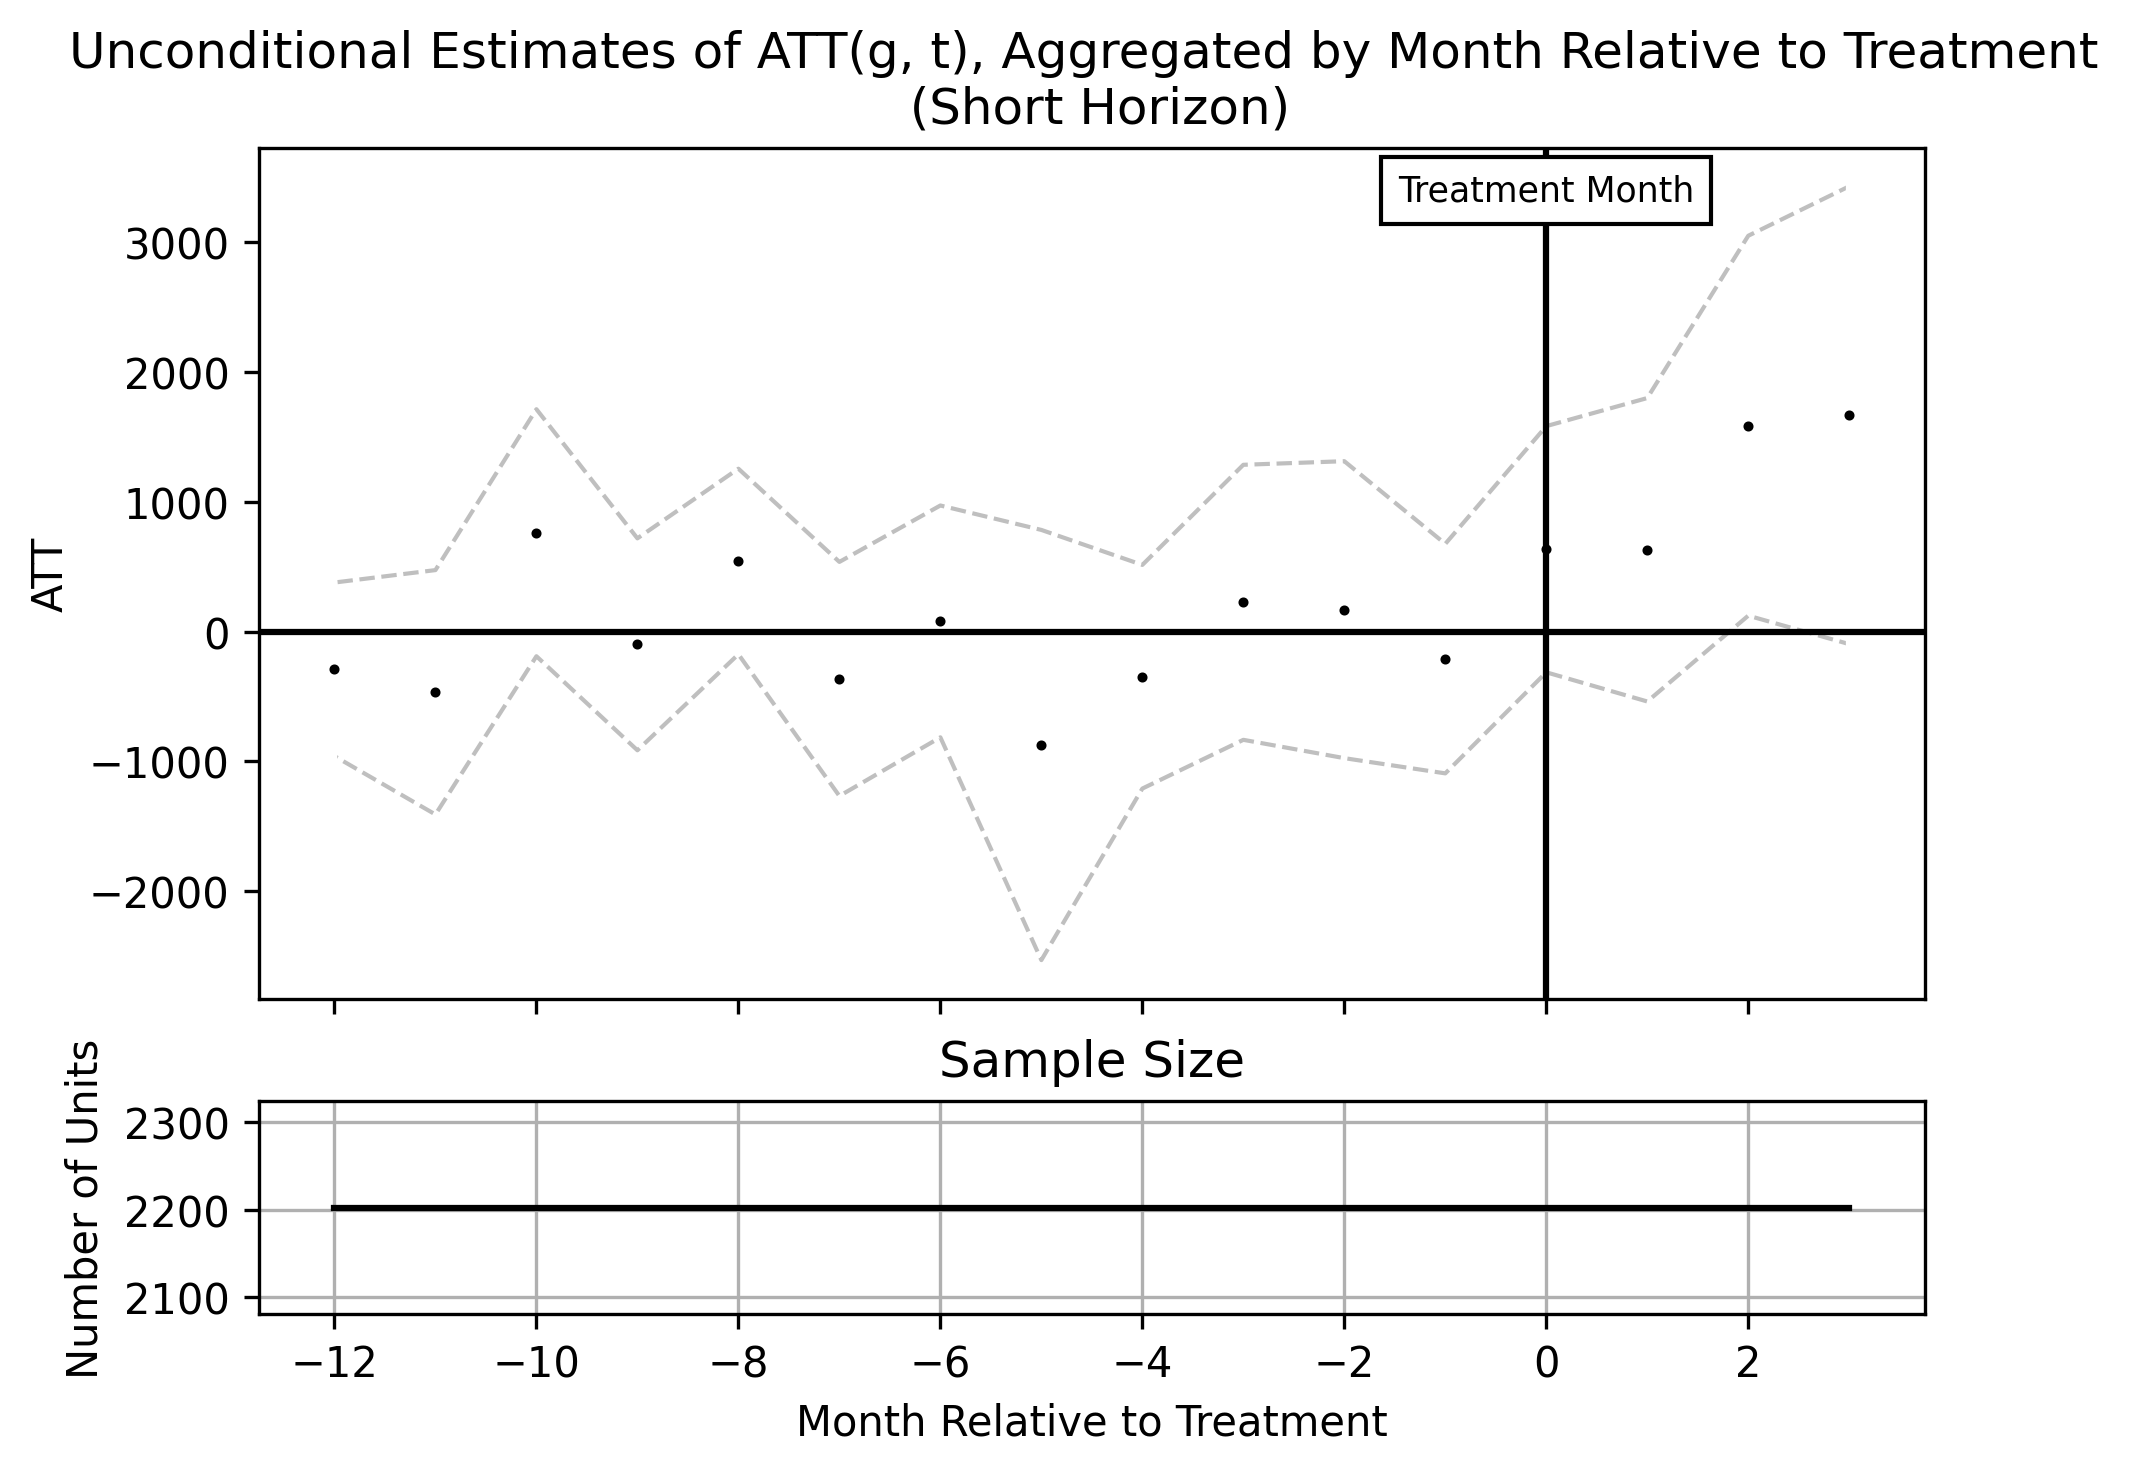
\includegraphics{output/DiD/figures/att_gt_unconditional_event_study_short_horizon.png}
        \caption{}
        \label{fig:my_label}
    \end{figure}

    \begin{figure}[H]
        \centering
        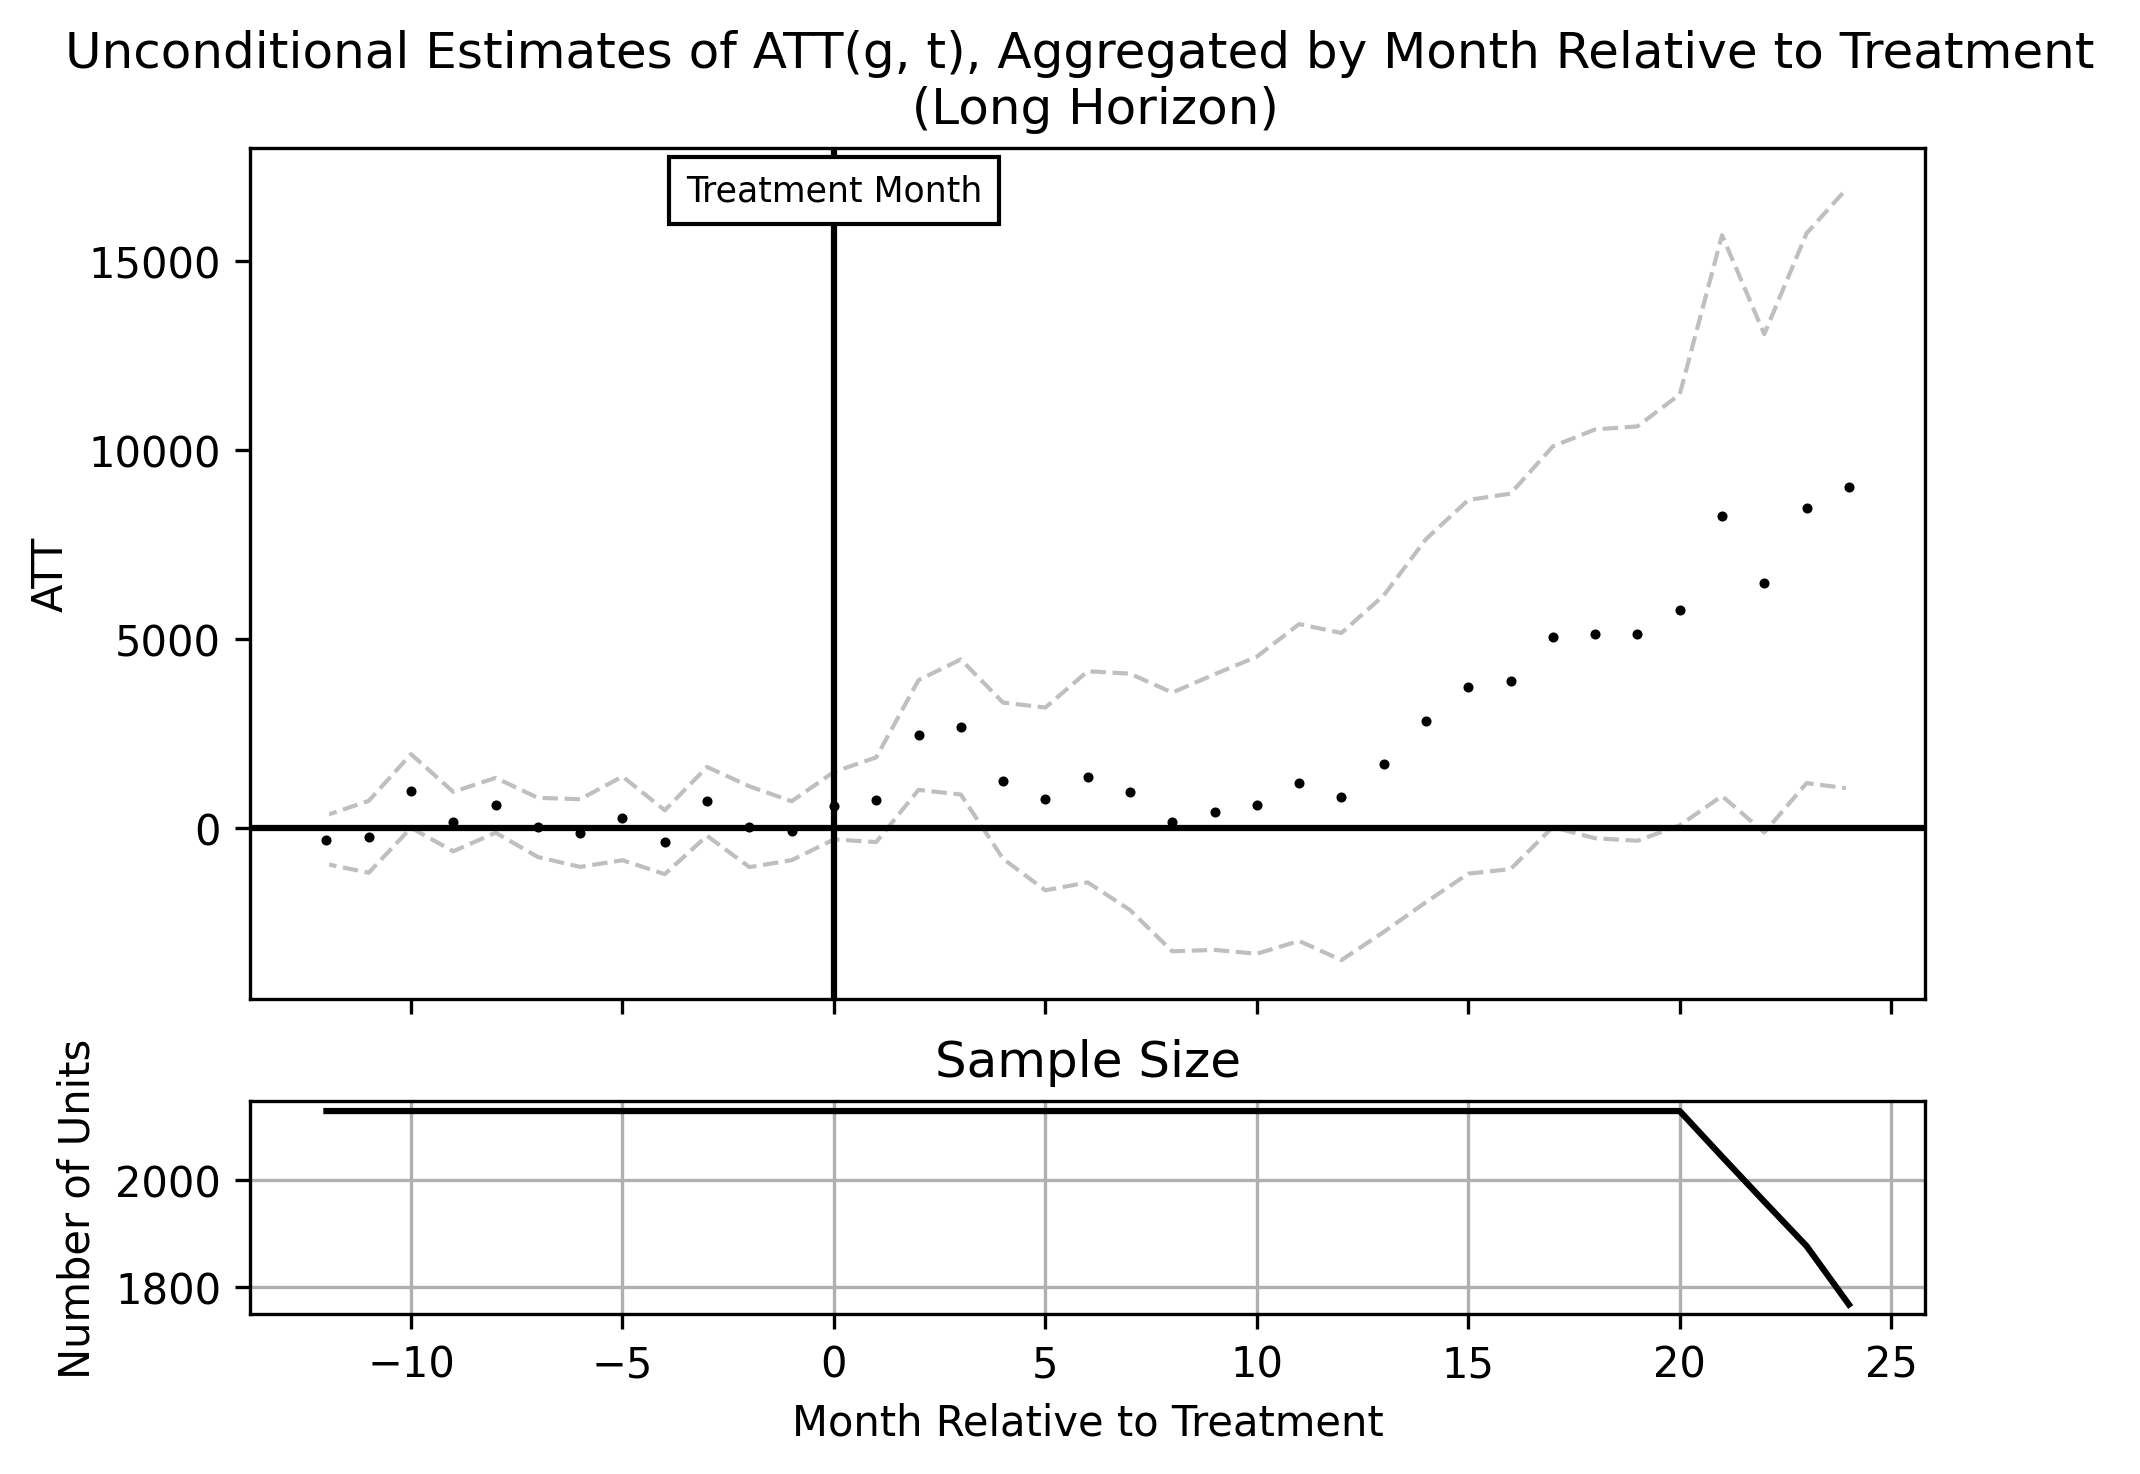
\includegraphics{output/DiD/figures/att_gt_unconditional_event_study_long_horizon.png}
        \caption{}
        \label{fig:my_label}
    \end{figure}
    
    \begin{figure}[H]
        \centering
        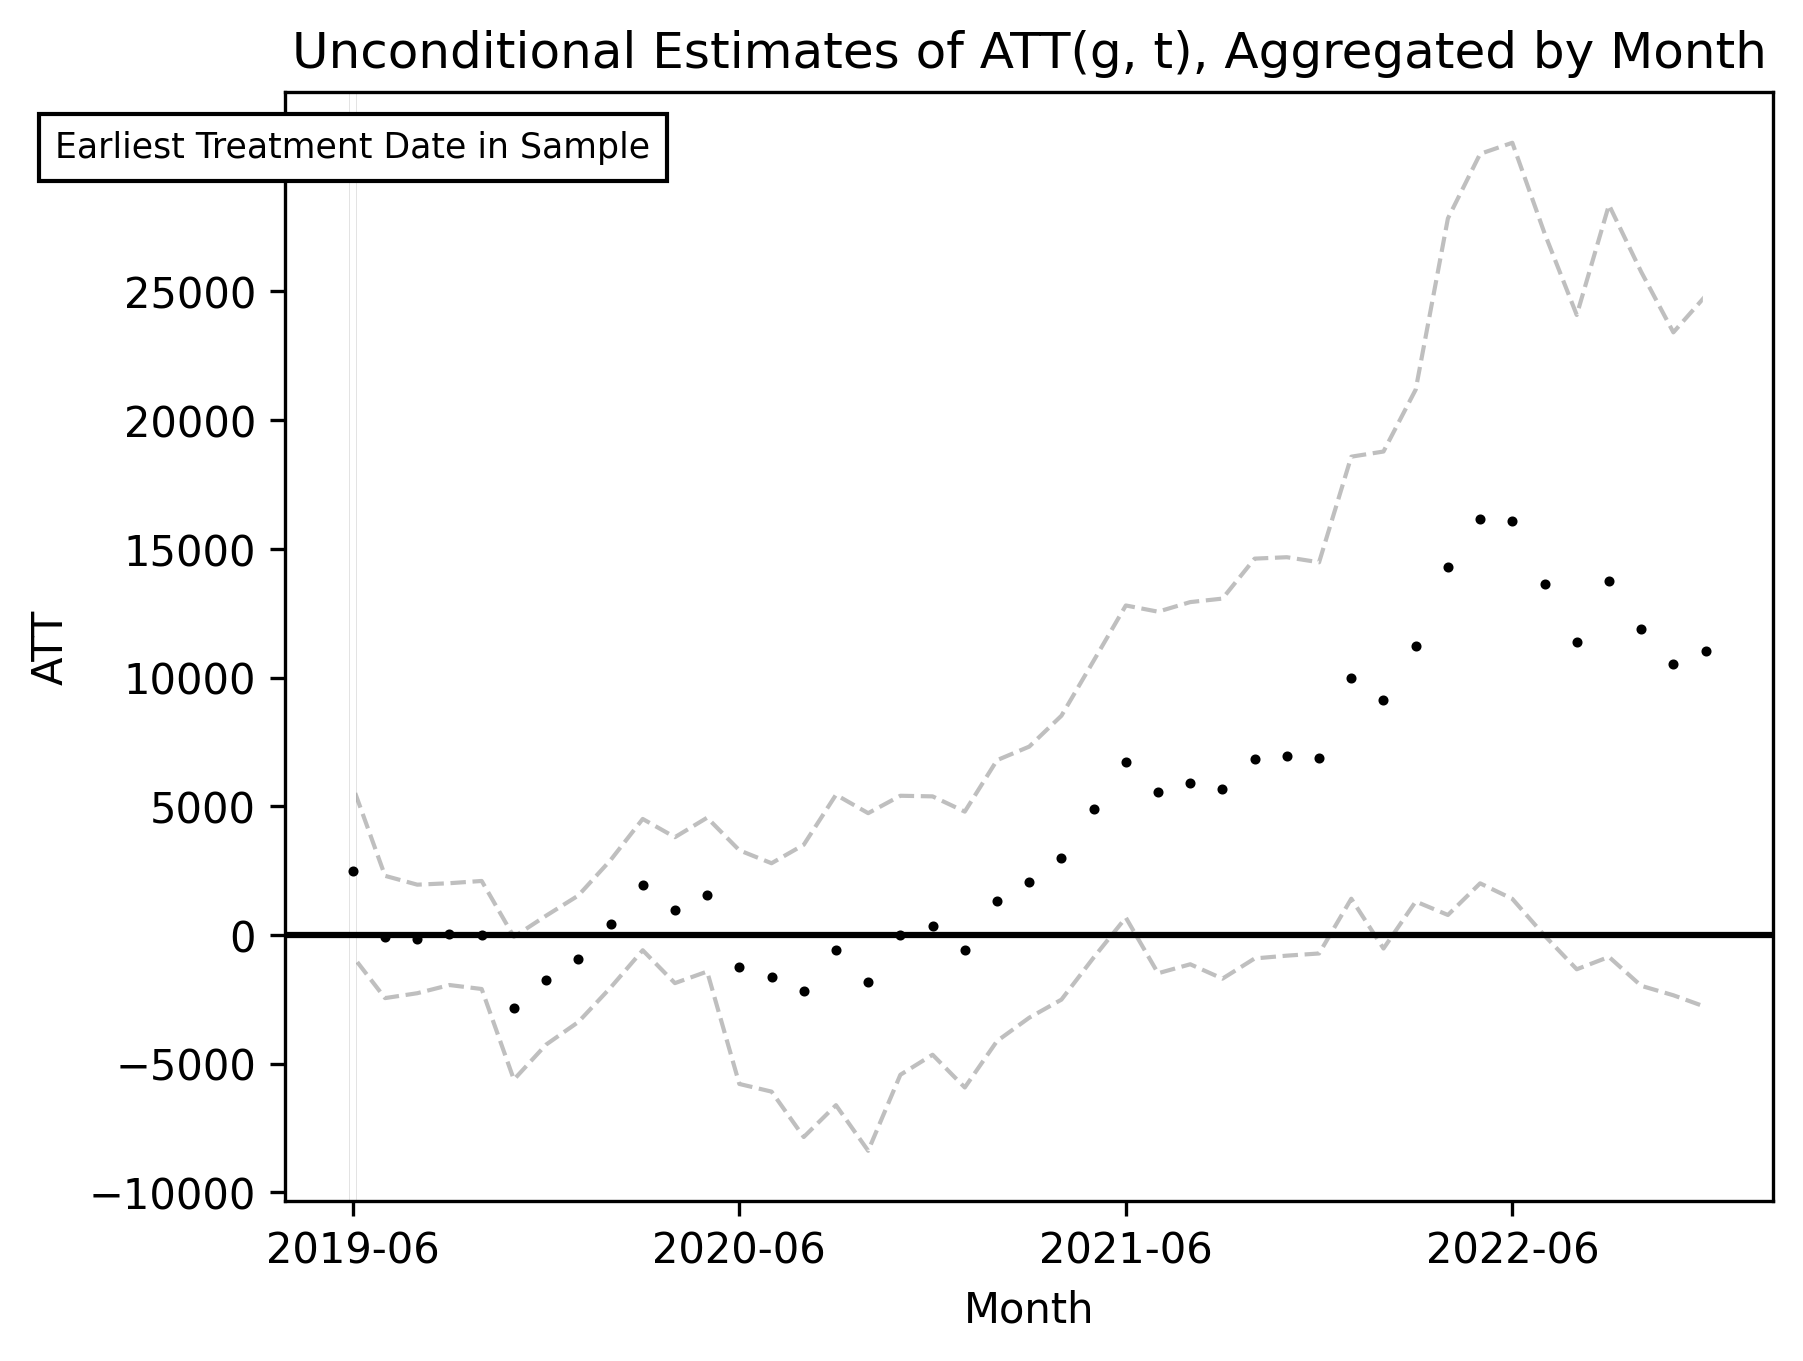
\includegraphics{output/DiD/figures/att_gt_unconditional_time.png}
        \caption{}
        \label{fig:my_label}
    \end{figure}

    \subsection{D.R. Estimates of the ATT}


    
    
    \begin{figure}[H]
        \centering
        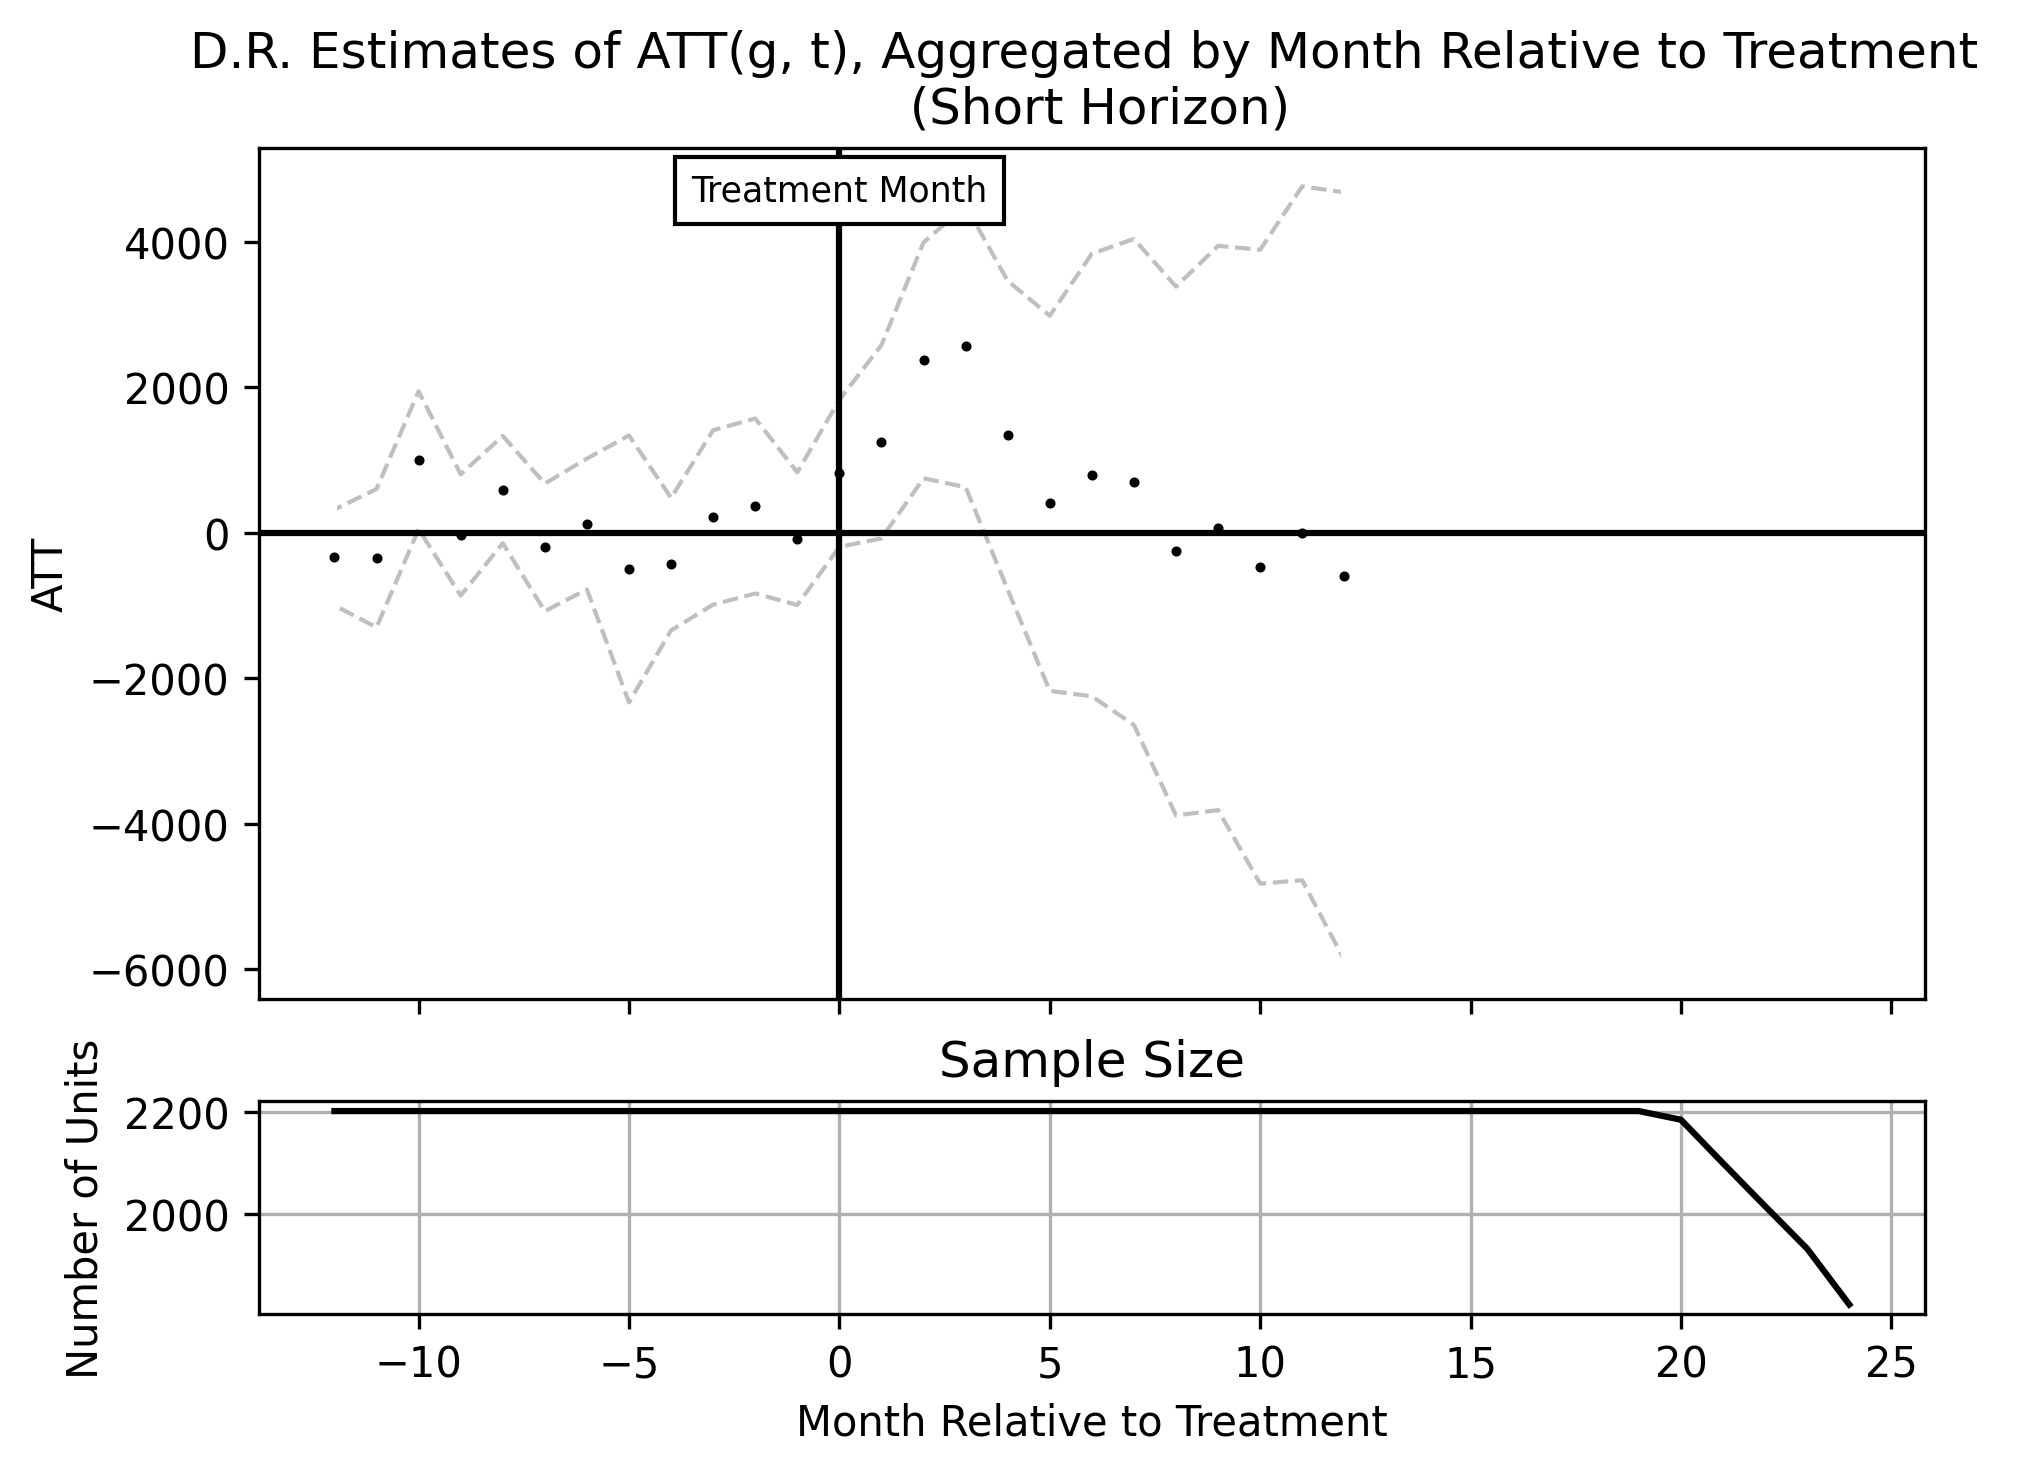
\includegraphics{output/DiD/figures/att_gt_dr_event_study_short_horizon.png}
        \caption{}
        \label{fig:my_label}
    \end{figure}
    
    \begin{figure}[H]
        \centering
        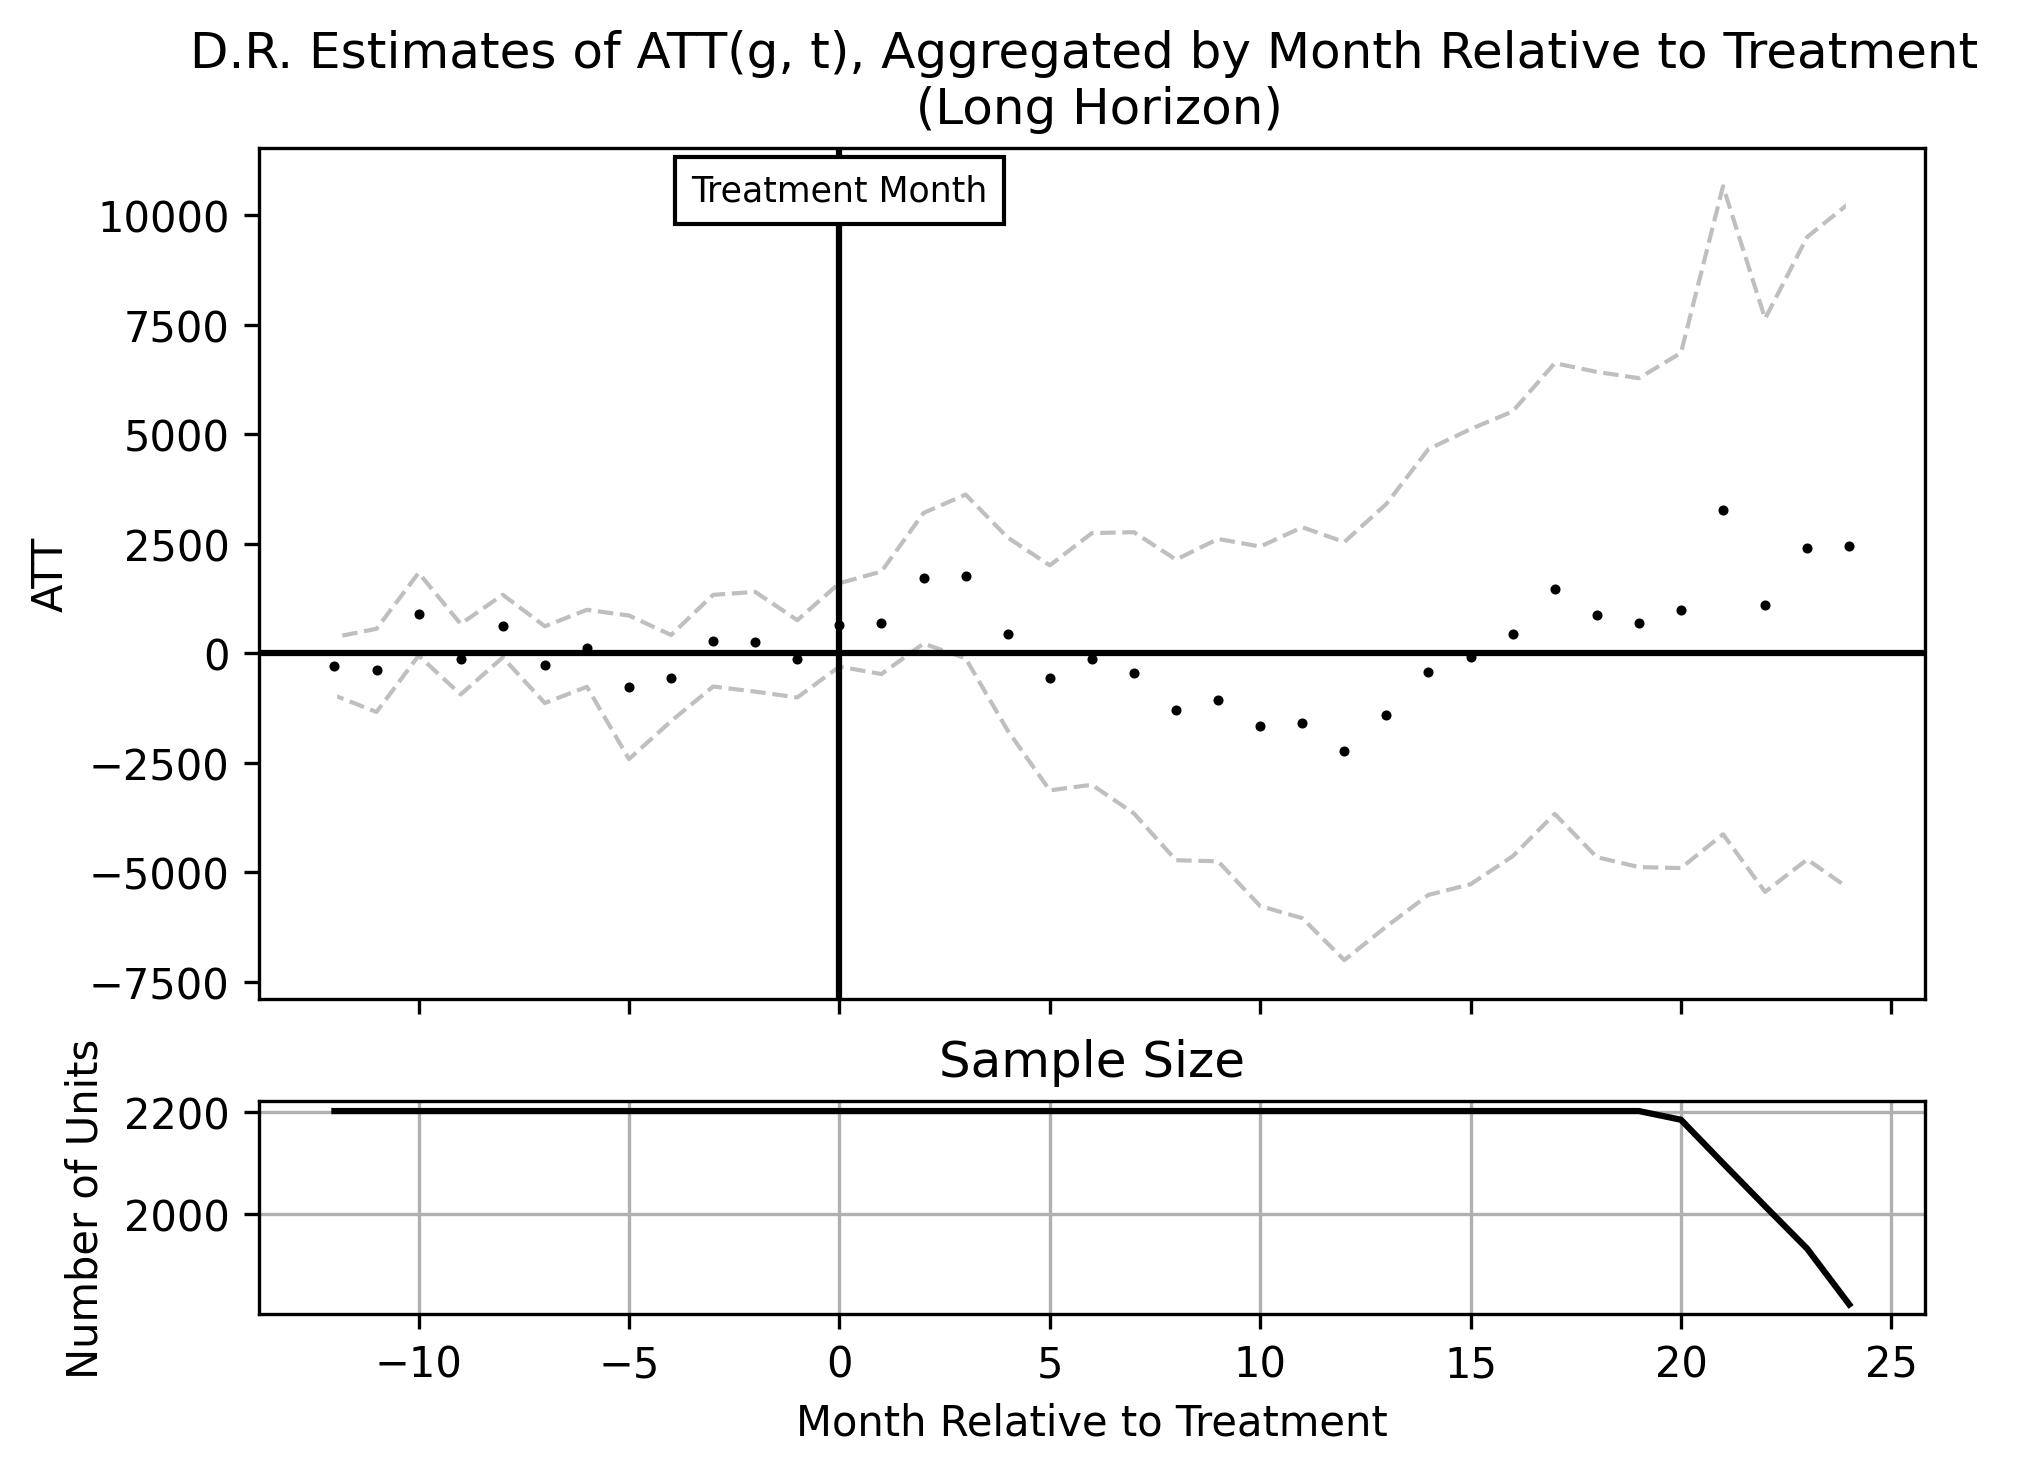
\includegraphics{output/DiD/figures/att_gt_dr_event_study_long_horizon.png}
        \caption{}
        \label{fig:my_label}
    \end{figure}

    \begin{figure}[H]
        \centering
        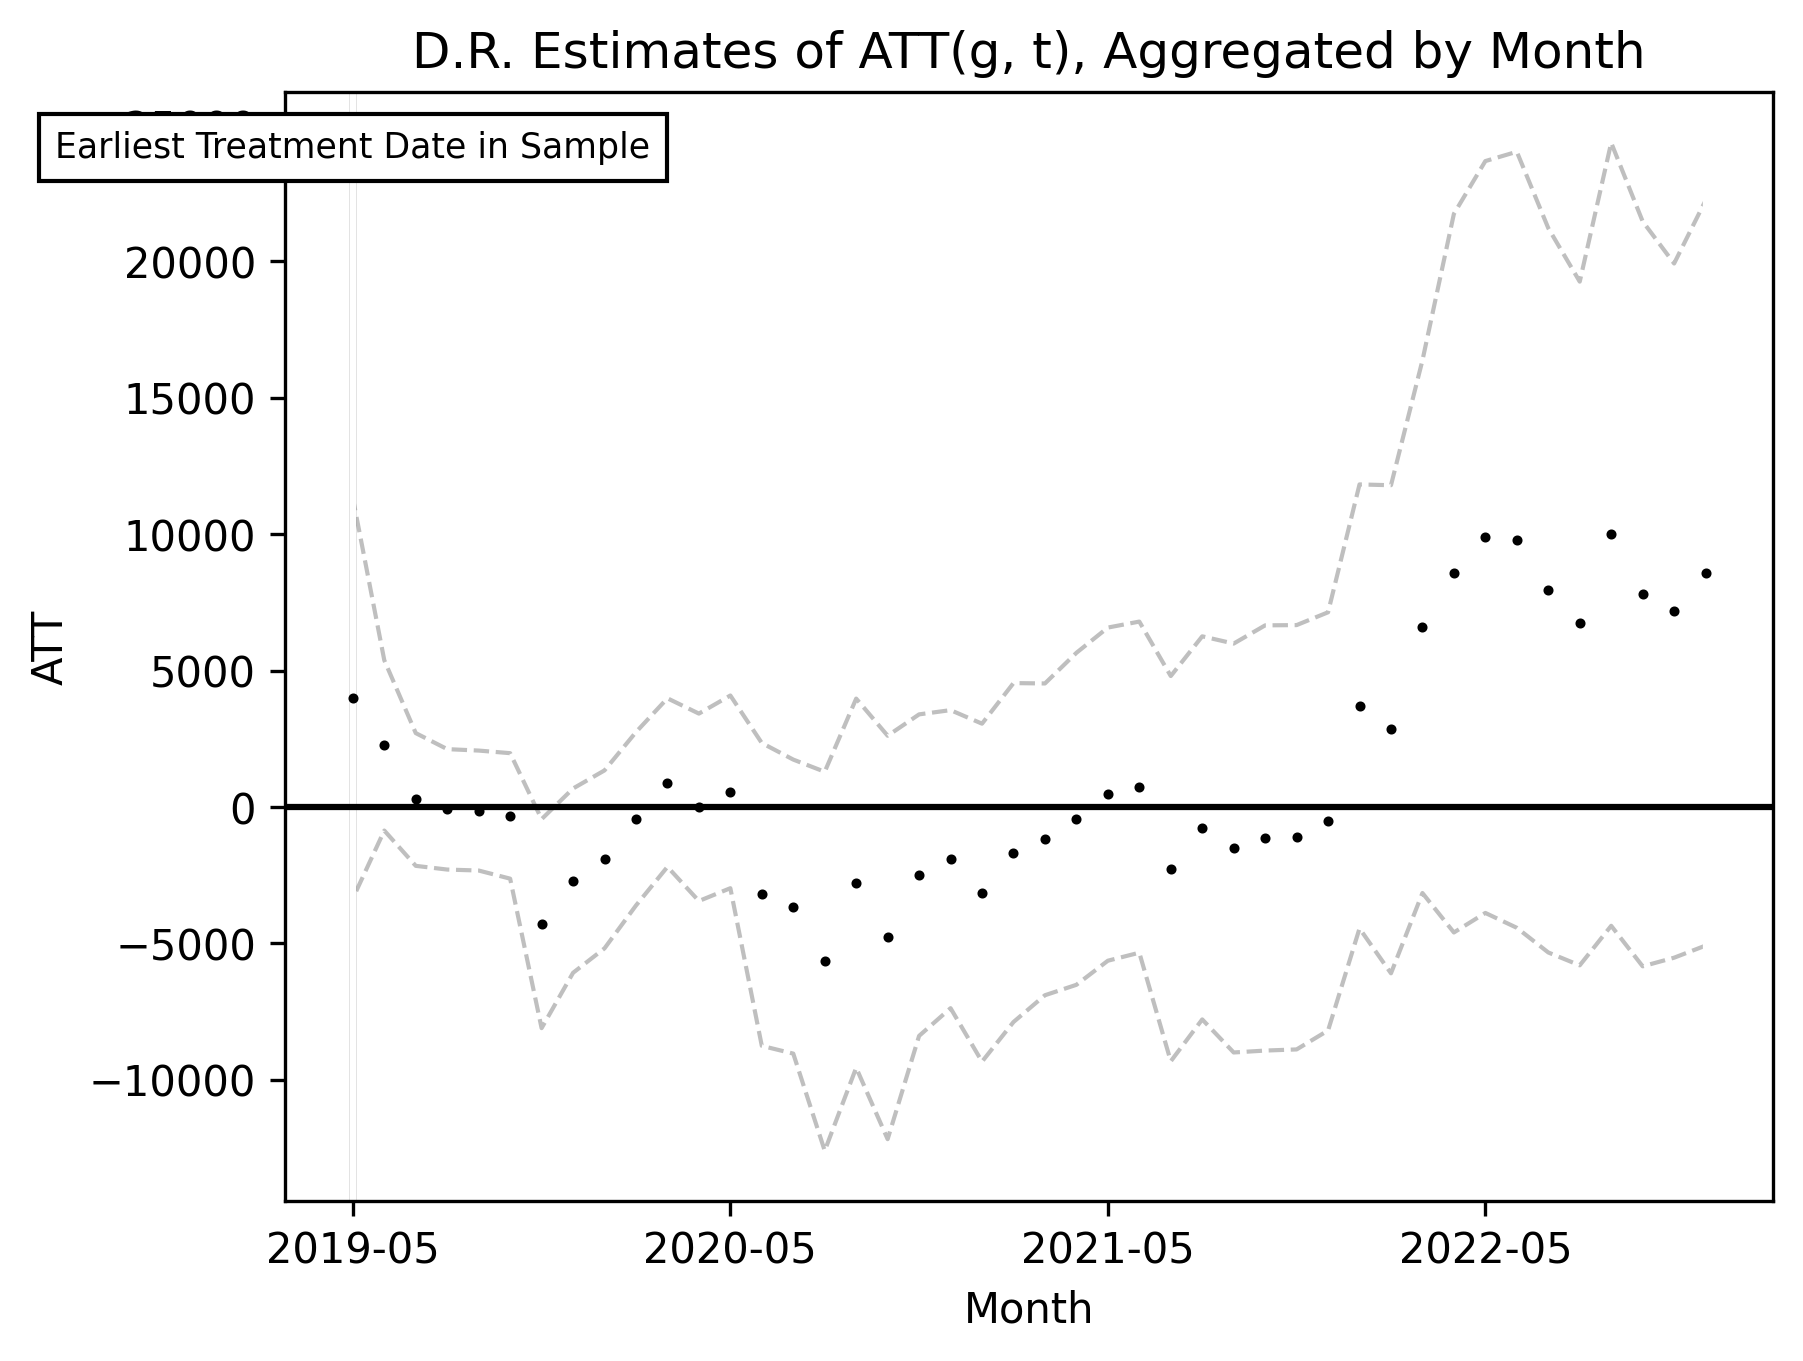
\includegraphics{output/DiD/figures/att_gt_dr_time.png}
        \caption{}
        \label{fig:my_label}
    \end{figure}


\section{Conclusion} \label{sec:conclusion}


\bibliography{citations}


\clearpage

\onehalfspacing

%
\end{document}